% Copyright 2004 by Till Tantau <tantau@users.sourceforge.net>.
%
% In principle, this file can be redistributed and/or modified under
% the terms of the GNU Public License, version 2.
%
% However, this file is supposed to be a template to be modified
% for your own needs. For this reason, if you use this file as a
% template and not specifically distribute it as part of a another
% package/program, I grant the extra permission to freely copy and
% modify this file as you see fit and even to delete this copyright
% notice. 

\documentclass{beamer}

% There are many different themes available for Beamer. A comprehensive
% list with examples is given here:
% http://deic.uab.es/~iblanes/beamer_gallery/index_by_theme.html
% You can uncomment the themes below if you would like to use a different
% one:
%\usetheme{AnnArbor}
%\usetheme{Antibes}
%\usetheme{Bergen}
%\usetheme{Berkeley}
%\usetheme{Berlin}
%\usetheme{Boadilla}
%\usetheme{boxes}
%\usetheme{CambridgeUS}
%\usetheme{Copenhagen}
%\usetheme{Darmstadt}
%\usetheme{default}
%\usetheme{Frankfurt}
%\usetheme{Goettingen}
%\usetheme{Hannover}
%\usetheme{Ilmenau}
%\usetheme{JuanLesPins}
%\usetheme{Luebeck}
\usetheme{Madrid}
%\usetheme{Malmoe}
%\usetheme{Marburg}
%\usetheme{Montpellier}
%\usetheme{PaloAlto}
%\usetheme{Pittsburgh}
%\usetheme{Rochester}
%\usetheme{Singapore}
%\usetheme{Szeged}
%\usetheme{Warsaw}
\graphicspath{{figures/}}
\definecolor{cwired}{rgb}{0.803,0.0,0.227}
\setbeamercolor{structure}{fg=cwired}
\title{Inverse Problems in Plasma Diffusion}

% A subtitle is optional and this may be deleted
\subtitle{A Probabilistic Approach for Physical Systems}

\author{Mandar ~Chandorkar}
% - Give the names in the same order as the appear in the paper.
% - Use the \inst{?} command only if the authors have different
%   affiliation.

\institute[CWI \& INRIA] % (optional, but mostly needed)
{
  \inst{1}%
  Multiscale Dynamics\\
  CWI, Amsterdam
  \and
  \inst{2}%
  TAO Research Unit\\
  INRIA, CNRS, Saclay}
% - Use the \inst command only if there are several affiliations.
% - Keep it simple, no one is interested in your street address.

\date{19 Sept 2017}
% - Either use conference name or its abbreviation.
% - Not really informative to the audience, more for people (including
%   yourself) who are reading the slides online

\subject{Machine Learning}
% This is only inserted into the PDF information catalog. Can be left
% out. 

% If you have a file called "university-logo-filename.xxx", where xxx
% is a graphic format that can be processed by latex or pdflatex,
% resp., then you can add a logo as follows:

% \pgfdeclareimage[height=0.5cm]{university-logo}{university-logo-filename}
% \logo{\pgfuseimage{university-logo}}

% Delete this, if you do not want the table of contents to pop up at
% the beginning of each subsection:
\AtBeginSubsection[]
{
  \begin{frame}<beamer>{Outline}
    \tableofcontents[currentsection,currentsubsection]
  \end{frame}
}

% Let's get started
\begin{document}

\begin{frame}
  \titlepage
\end{frame}

\begin{frame}{Outline}
  \tableofcontents
  % You might wish to add the option [pausesections]
\end{frame}

% Section and subsections will appear in the presentation overview
% and table of contents.
\section{Problem}

\subsection{Magnetosphere}

\begin{frame}
  \begin{figure}[h]
        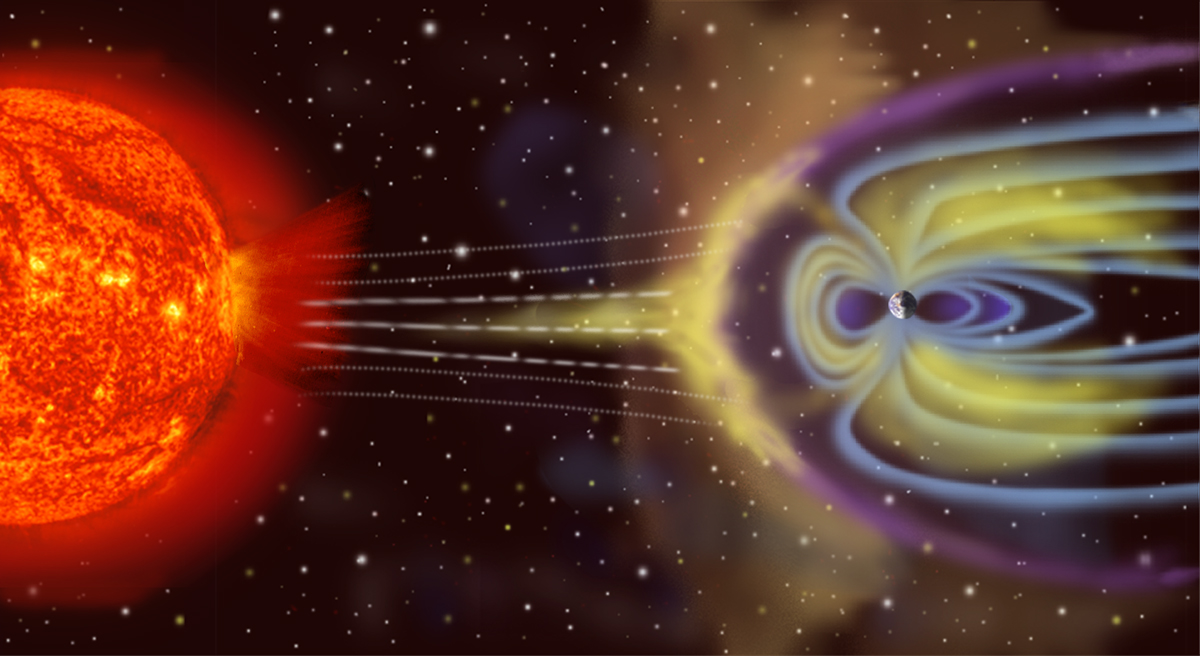
\includegraphics[width=0.8\textwidth]{Magnetosphere_rendition}
        \caption{Sun-Magnetosphere System}
        \label{fig:Solar}
      \end{figure}
\end{frame}

\begin{frame}{Radiation Belts}
  \textbf{Van Allen radiation belts} are a layer of trapped charged particles around the Earth.
  \begin{itemize}
  \item {
      \textbf{Outer radiation belt}, mainly composed of high energy electrons (energetic range around 0.1 to 10 MeV)
  }
  \item {
      \textbf{Inner radiation belt}, composed of high concentrations of electrons (energetic range of hundreds of keV) and energetic protons.
  }
  \end{itemize}
\end{frame}

\subsection{Plasma Dynamics:  Adiabatic Theory}

% You can reveal the parts of a slide one at a time
% with the \pause command:
\begin{frame}{Plasma Motions}

  Motion of charged particles is decomposed into three components.
  
   \begin{figure}[h]
        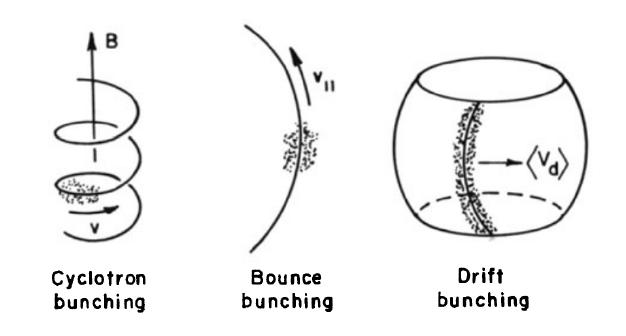
\includegraphics[width=0.5\textwidth]{adiabatic_motions}
        \caption{Adiabatic Motions}
        \label{fig:Adiabatic}
      \end{figure}
\end{frame}

\begin{frame}{Adiabatic Invariants}
  For each component of plasma motion, there is one \emph{adiabatic
    invariant} associated.

  \begin{itemize}
  \item<1->{
      Cyclotron Motion: $M$
    }
  \item<2->{
      Bounce Motion: $J$
    }
  \item<3->{
      Drift Motion: $\Phi$
    }
  \end{itemize}

\end{frame}

\subsection{Plasma Dynamics: Diffusion Theory}

\begin{frame}{Radial Diffusion}
  \begin{equation}
    \frac{\partial{f}}{\partial{t}} = l^2 \left( \frac{\kappa(l,
        t)}{l^{2}} \frac{\partial{f}}{\partial{l}} \right) - \lambda(l,
    t) f +  Q(l, t)
  \end{equation}

  
\end{frame}

\begin{frame}{Key Quantities}
  \begin{itemize}
  \item {
      $f$: Plasma \emph{phase space density}
    \pause % The slide will pause after showing the first item
  }
  \item {   
      $\kappa(l, t)$: Diffusion field.
  }
  % You can also specify when the content should appear
  % by using <n->:
  \item<3-> {
    $\lambda(l, t)$: Particle loss rate.
  }
  \item<4-> {
      $Q(l, t)$: Particle injection rate (Shall be set to zero for
      in context).
  }
  \end{itemize}
\end{frame}

\subsection{Parameter Estimation}


\section{Methodology}



\begin{frame}{Blocks}
\begin{block}{Block Title}
You can also highlight sections of your presentation in a block, with it's own title
\end{block}
\begin{theorem}
There are separate environments for theorems, examples, definitions and proofs.
\end{theorem}
\begin{example}
Here is an example of an example block.
\end{example}
\end{frame}

% Placing a * after \section means it will not show in the
% outline or table of contents.
\section*{Summary}

\begin{frame}{Summary}
  \begin{itemize}
  \item
    The \alert{first main message} of your talk in one or two lines.
  \item
    The \alert{second main message} of your talk in one or two lines.
  \item
    Perhaps a \alert{third message}, but not more than that.
  \end{itemize}
  
  \begin{itemize}
  \item
    Outlook
    \begin{itemize}
    \item
      Something you haven't solved.
    \item
      Something else you haven't solved.
    \end{itemize}
  \end{itemize}
\end{frame}



% All of the following is optional and typically not needed. 
\appendix
\section<presentation>*{\appendixname}
\subsection<presentation>*{For Further Reading}

\begin{frame}[allowframebreaks]
  \frametitle<presentation>{For Further Reading}
    
  \begin{thebibliography}{10}
    
  \beamertemplatebookbibitems
  % Start with overview books.

  \bibitem{Author1990}
    A.~Author.
    \newblock {\em Handbook of Everything}.
    \newblock Some Press, 1990.
 
    
  \beamertemplatearticlebibitems
  % Followed by interesting articles. Keep the list short. 

  \bibitem{Someone2000}
    S.~Someone.
    \newblock On this and that.
    \newblock {\em Journal of This and That}, 2(1):50--100,
    2000.
  \end{thebibliography}
\end{frame}

\end{document}


